\documentclass[UTF8,openany,AutoFakeBold,zihao=-4,screen]{ctexbook}
% ↑ 打印前去除screen选项,以应用奇偶页不对称(装订线5mm)的排版效果

\makeatletter
\newif\ifscreen
\@ifclasswith{ctexbook}{screen}{\screentrue}{\screenfalse}
\makeatother

\ifscreen
    \usepackage[a4paper,left=2.25cm,right=2.25cm,top=2.5cm,bottom=2.5cm]{geometry}
\else
    \usepackage[a4paper,left=2.5cm,right=2cm,top=2.5cm,bottom=2.5cm,twoside]{geometry}
\fi

\makeatletter
\def\emptypage@emptypage{%
    \hbox{}%
     \vspace*{\fill}
     \begin{center}
        % 打印前请去除documentclass的screen选项,去除后将不再显示此文字
        \ifscreen{\small(此页为空白页)}\fi
     \end{center}
     \vspace{\fill}
     \newpage%
}%
\def\cleardoublepage{%
        \clearpage%
        \if@twoside%
            \ifodd\c@page%
                % do nothing
            \else%
                \emptypage@emptypage%
            \fi%
        \fi%
    }%
\makeatother

\usepackage{algorithmic}
\usepackage[ruled,linesnumbered,vlined]{algorithm2e}
\usepackage{subcaption}
\usepackage{url}
\usepackage{calc}
\usepackage{amsmath}
\usepackage{amssymb}
\usepackage{bm}
\usepackage{amsfonts}
\usepackage{enumerate}
\usepackage{fancyhdr}
\usepackage[super,square,sort,compress]{natbib}
\usepackage{multirow,booktabs,makecell}
\usepackage{graphicx}
\usepackage{datetime2}
\usepackage[font=small,labelsep=space]{caption} %五号,宋体/Time new roman
%\renewcommand{\thetable}{\arabic{table}} %表格和图片编号不分章节,直接1,2,3 ...
%\renewcommand{\thefigure}{\arabic{figure}}
\renewcommand{\theequation}{\arabic{chapter}.\arabic{equation}} %公式标签 章.公式(均为阿拉伯数字)

\ifscreen
    \usepackage[colorlinks,allcolors=violet]{hyperref}
\else
    \usepackage[hidelinks]{hyperref}
\fi

\usepackage{enumitem}
\setlist{nosep}
\setlist[1]{leftmargin=3em}

% below: circled footnote symbols
\usepackage{pifont}
\usepackage[perpage,symbol*]{footmisc}
\DefineFNsymbols{circled}{{\ding{192}}{\ding{193}}{\ding{194}}{\ding{195}}{\ding{196}}{\ding{197}}{\ding{198}}{\ding{199}}{\ding{200}}{\ding{201}}}
\setfnsymbol{circled}
% below: normal number size in footnote
\makeatletter
\long\def\@makefntext#1{\noindent{{\@thefnmark}\enskip #1}}
\makeatother

\usepackage{tocloft} %自定义目录,说明中没有明确规定,和WORD自动生成目录格式一致

%“目录”两个字的格式
\renewcommand\cftbeforetoctitleskip{0pt}
\renewcommand\cftaftertoctitleskip{0pt}
\renewcommand\cfttoctitlefont{\bfseries\heiti\zihao{2}}

% below: toc styles

\cftsetpnumwidth{1em}

\renewcommand\cftchapfont{\heiti\small}
\renewcommand\cftchapleader{\cftdotfill{\cftchapdotsep}}
\renewcommand\cftchapdotsep{1}
\setlength{\cftchapnumwidth}{1em}
\renewcommand\cftchappagefont{\songti\small}
\renewcommand\cftbeforechapskip{0pt}

\renewcommand\cftsecfont{\songti\small}
\renewcommand\cftsecdotsep{1}
\setlength{\cftsecnumwidth}{1em}
\renewcommand\cftsecpagefont{\songti\small}
\renewcommand\cftsecindent{1em}
\renewcommand\cftbeforesecskip{0pt}

\renewcommand\cftsubsecfont{\songti\small}
\renewcommand\cftsubsecdotsep{1}
\setlength{\cftsubsecnumwidth}{1em}
\renewcommand\cftsubsecpagefont{\songti\small}
\renewcommand\cftsubsecindent{2em}
\renewcommand\cftbeforesubsecskip{0pt}

\renewcommand\cftsubsubsecfont{\songti\small}
\renewcommand\cftsubsubsecdotsep{1}
\setlength{\cftsubsubsecnumwidth}{1em}
\renewcommand\cftsubsubsecpagefont{\songti\small}
\renewcommand\cftsubsubsecindent{3em}
\renewcommand\cftbeforesubsubsecskip{0pt}

\usepackage{titlesec}%自定义章节标题
\ctexset{
    chapter = {
        format={\center \heiti \zihao {3}},
        beforeskip=0pt 
    }
}

\setcounter{tocdepth}{3}
\setcounter{secnumdepth}{3}
%使目录中有三级标题,即subsubsection

% below: section title fonts
\titleformat{\section}{\raggedright\zihao{3}\songti}{\thesection\quad}{0pt}{}
\titleformat{\subsection}{\raggedright\zihao{4}\songti}{\thesubsection\quad}{0pt}{}
\titleformat{\subsubsection}{\raggedright\zihao{-4}\songti}{\thesubsubsection\quad}{0pt}{}

\input{head/CoverHead}
\input{head/ReviewTableHead}

\input{includes}
\newcommand{\chineseTitleA}{随机测试用例排序的}
\newcommand{\chineseTitleB}{一个理论分析}
\newcommand{\englishTitleA}{A Theoretical Analysis of Random}
\newcommand{\englishTitleB}{Regression Test Prioritization}
\newcommand{\name}{易普}
\newcommand{\studentID}{1800013116}
\newcommand{\school}{信息科学技术学院(本科生学院)}
\newcommand{\major}{计算机科学与技术}
\newcommand{\advisor}{谢涛}
\newcommand{\advisorAffiliation}{软件研究所}
\newcommand{\advisorTitle}{讲席教授}



\newcommand{\Comment}[1]{}
\newcommand{\Fix}[1]{\textbf{[[#1]]}}
\newcommand{\testcase}{test\Space{ case}}
\newcommand{\Testcase}{Test\Space{ case}}
\newcommand{\order}{order\Space{ing}}

\newcommand{\CodeIn}[1]{{\small\texttt{#1}}}

\newcommand{\ccc}[1]{\hfill\begin{scriptsize}// \textrm{#1}\end{scriptsize}}
\newcommand{\Output}{p}
\newcommand{\pmfKey}{x}
\newcommand{\pmfSet}{\mathcal{P}}
\newcommand{\twoParaFunc}[3]{\ensuremath{\mathrm{#1_{#2,#3}}}}
\newcommand{\individualreview}[1]{{\color{individualColor} #1}}
\newcommand{\reviewcomments}[1]{}

\newcommand{\Space}[1]{}
\newcommand{\Num}[1]{#1}

\def\z{\phantom{0}}

\newcommand{\idflakies}{iDFlakies\xspace}
\newcommand{\percIdflakiesOD}{50.5\%\xspace}
\newcommand{\percIdflakiesNOD}{49.5\%\xspace}

\newcommand{\comprehensive}{comprehensive\xspace}
\newcommand{\extended}{extended\xspace}

\newcommand{\originalConfig}{original-order\xspace}
\newcommand{\randomClass}{random-class\xspace}
\newcommand{\randomClassAbb}{RandomC\xspace}
\newcommand{\randomClassMethod}{random-class-method\xspace}
\newcommand{\randomClassMethodAbb}{RandomC+M\xspace}
\newcommand{\reverseClassMethod}{reverse-class-method\xspace}
\newcommand{\reverseClassMethodAbb}{ReverseC+M\xspace}
\newcommand{\reverseClass}{reverse-class\xspace}
\newcommand{\reverseClassAbb}{ReverseC\xspace}

\newcommand{\interleavingFull}{Interleavings\xspace}
\newcommand{\junitFull}{Groupings\xspace}
\newcommand{\interleaving}{``I''\xspace}
\newcommand{\junit}{``G''\xspace}

\newcommand{\cleaner}{cleaner\xspace}
\newcommand{\polluter}{polluter\xspace}
\newcommand{\statesetter}{state-setter\xspace}
\newcommand{\brittle}{brittle\xspace}
\newcommand{\victim}{victim\xspace}
\newcommand{\cleaners}{cleaners\xspace}
\newcommand{\polluters}{polluters\xspace}
\newcommand{\statesetters}{state-setters\xspace}
\newcommand{\brittles}{brittles\xspace}
\newcommand{\victims}{victims\xspace}

\newcommand{\Cleaner}{Cleaner\xspace}
\newcommand{\Polluter}{Polluter\xspace}
\newcommand{\Statesetter}{State-setter\xspace}
\newcommand{\Brittle}{Brittle\xspace}
\newcommand{\Victim}{Victim\xspace}
\newcommand{\Cleaners}{Cleaners\xspace}
\newcommand{\Polluters}{Polluters\xspace}
\newcommand{\Statesetters}{State-setters\xspace}
\newcommand{\Brittles}{Brittles\xspace}
\newcommand{\Victims}{Victims\xspace}

% ======== Practical RTP 
\newcommand{\classInterleave}{CAM\xspace}
\newcommand{\methodInterleave}{MAC\xspace}
\newcommand{\classInterleaveLONG}{classes across modules\xspace}
\newcommand{\methodInterleaveLONG}{methods across classes\xspace}
\newcommand{\MethodInterleaveLONG}{Methods Across Classes\xspace}
\newcommand{\testprioritization}{test prioritization\xspace}

\newcommand{\APFD}{\ensuremath{\mathrm{\alpha}}}
\newcommand{\APFDc}{\ensuremath{\mathrm{\gamma}}}
\newcommand{\APFDfor}[1]{\APFD(#1)}
\newcommand{\APFDcfor}[1]{\APFDc(#1)}

\newcommand{\APFDcFull}{\ensuremath{\mathrm{\ensuremath{\mathrm{APFD}_c}}}}
\newcommand{\APFDFull}{\ensuremath{\mathrm{\ensuremath{\mathrm{APFD}}}}}

\newcommand{\mappingOneToOne}{one-to-one\xspace}
\newcommand{\mappingAllToOne}{all-to-one\xspace}
\newcommand{\mappingModToOne}{module-to-one\xspace}

\newcommand{\MappingOneToOne}{One-to-one\xspace}
\newcommand{\MappingAllToOne}{All-to-one\xspace}
\newcommand{\MappingModToOne}{Module-to-one\xspace}

\newcommand{\RTP}{RTP}
\newcommand{\TCP}{RTP}

% ======== Misc
\newcommand{\strategy}{technique}

\newcommand{\testmethods}{\Space{test m}methods\xspace}
\newcommand{\Testmethods}{\Space{Test m}Methods\xspace}
\newcommand{\testclasses}{\Space{test c}classes\xspace}
\newcommand{\Testclasses}{\Space{Test c}Classes\xspace}

\newcommand{\testmethod}{\Space{test m}method\xspace}
\newcommand{\Testmethod}{\Space{Test m}Method\xspace}
\newcommand{\testclass}{\Space{test c}class\xspace}
\newcommand{\Testclass}{\Space{Test c}Class\xspace}

\newcommand{\approaches}{approaches\xspace}
\newcommand{\approach}{approach\xspace}

% for figures
\newcommand{\precaptionspace}{\vspace{-3ex}}
% for tables
\newcommand{\pretabcaptionspace}{\vspace*{-1.5ex}}
\newcommand{\posttabcaptionspace}{\vspace*{-1.5ex}}

\newcommand{\detect}{检测\xspace}
\newcommand{\detects}{检测\xspace}
\newcommand{\detected}{detected\xspace}
\newcommand{\detecting}{detecting\xspace}
\newcommand{\detectors}{detectors\xspace}
\newcommand{\detector}{detector\xspace}
\newcommand{\undetected}{undetected\xspace}

\newcommand{\introduced}{added\xspace}
\newcommand{\numApproaches}{two\xspace}

\newcommand{\kind}{kind\xspace}
\newcommand{\kinds}{kinds\xspace}

\newcommand{\classification}{categorization\xspace}
\newcommand{\classify}{categorize\xspace}
\newcommand{\classifies}{categorizes\xspace}
\newcommand{\classified}{categorized\xspace}
\newcommand{\Classifying}{Categorizing\xspace}
\newcommand{\classifying}{categorizing\xspace}

\newcommand{\priorFlakyClaim}{78\%\xspace}
\newcommand{\Project}[1]{\CodeIn{#1}}

\newcommand{\framework}{framework\xspace}
\newcommand{\Framework}{Framework\xspace}

\newcommand{\configuration}{configuration\xspace}
\newcommand{\configurations}{configurations\xspace}
\newcommand{\Configurations}{Configurations\xspace}

\newcommand{\cmark}{\ding{51}}
\newcommand{\xmark}{\ding{55}}

{\makeatletter
 \gdef\jonmark{
   \expandafter\ifx\csname @mpargs\endcsname\relax
     \expandafter\ifx\csname @captype\endcsname\relax
       \marginpar{\textcolor{blue}{jon~}}
     \else
       \textcolor{blue}{jon~}
     \fi
   \else
     \textcolor{blue}{jon~}
   \fi}
 \gdef\jon{\@ifnextchar[\tianyin@lab\jon@nolab}
 \long\gdef\jon@lab[#1]#2{{\bf [\jonmark \textcolor{blue}{#2} ---{\sc #1}]}}
 \long\gdef\jon@nolab#1{{\bf [\jonmark \textcolor{blue}{Jon: #1}]}}
}


\newcommand{\Def}[2]{\expandafter\newcommand\csname rmk-#1\endcsname{#2}}
\newcommand{\Use}[1]{\csname rmk-#1\endcsname}

\newcommand{\category}{category\xspace}
\newcommand{\Category}{Category\xspace}
\newcommand{\categories}{categories\xspace}
\newcommand{\Categories}{Categories\xspace}
\newcommand{\categorize}{categorize\xspace}
\newcommand{\Categorize}{Categorize\xspace}

\newcommand{\Prob}[1]{P(#1)}
\newcommand{\Proba}[1]{P_a(#1)}
\newcommand{\Probn}[1]{P_c(#1)}
\newcommand{\allordersubscript}{_a}
\newcommand{\ccordersubscript}{_c}
\newcommand{\E}[1]{\mathrm{E}[#1]}
\newcommand{\Ea}[1]{\mathrm{E\allordersubscript}[#1]}
\newcommand{\En}[1]{\mathrm{E\ccordersubscript}[#1]}
\newcommand{\Cost}[1]{\sigma(#1)}
\newcommand{\Costo}[1]{\sigma_o(#1)}
\newtheorem{mytheorem}{\setcounter{corollary}{1}Theorem}
\newtheorem{mycorollary}{Corollary}[mytheorem]
\renewcommand{\themycorollary}{\themytheorem.\arabic{corollary}}
\newtheorem{mylemma}[mytheorem]{Lemma}
\newtheorem{mydefinition}[mytheorem]{Definition}

\newcommand{\etal}{et al.\xspace}

\newcommand{\simulated}{simulated\xspace}

\newcommand{\Answer}[2]{\noindent \textbf{A#1:} #2}

\newcommand{\currentYear}{2022}

\newcommand{\maxNumberOfTests}{2118}
\newcommand{\maxNumberOfFailures}{372}

\newcommand{\testClassInFormula}{C}
\newcommand{\classSet}{\ensuremath{\mathcal{\testClassInFormula}}}
\newcommand{\TF}{\ensuremath{\tau}}

\newcommand{\plotscale}{1}

\newcommand{\reverseOrder}[1]{\overline{#1}}

\newcommand{\mappingMatrix}{失败-缺陷映射矩阵\xspace}
\newcommand{\mappingMatrices}{失败-缺陷映射矩阵\xspace}

\newcommand{\compatible}{兼容}
\newcommand{\Compatible}{兼容}
\newcommand{\cOmpatible}{兼容}
\newcommand{\zeroFunction}{\mathbf{zero}}
\newcommand{\mappingRelation}{\mu}

\newcommand{\distributions}{PMFs\xspace}
\newcommand{\distribution}{PMF\xspace}
\newcommand{\Distribution}{PMF\xspace}
\newcommand{\Distributions}{PMFs\xspace}

\newcommand{\undetectedFaults}{UF}
\newcommand{\failingTests}{FT}
\newcommand{\faultsDetected}{FD}
\newcommand{\newRelation}{NR}

\newcommand{\proxyVariable}{V(n,\mappingRelation)}
\newcommand{\position}{\ensuremath{\phi}}

\newcommand{\CPPLine}{117\xspace}
\newcommand{\mean}[1]{\Ea{#1}}
\newcommand{\median}[1]{\mathrm{Med_a}(#1)}

\newcommand{\Omitted}[1]{\emph{Omitted for space reasons.}}

\newcommand{\formula}[1]{(\ref{#1})}

\newcommand{\litReviewCompareYes}{56\xspace}
\newcommand{\litReviewCompareNO}{44\xspace}
\newcommand{\litReviewPlotsYes}{40\Fix{Wing needs to double check}\xspace}
\newcommand{\litReviewPlotsNO}{16\xspace}
\newcommand{\litReviewSuspYes}{8\xspace}
\newcommand{\litReviewSuspNO}{32\xspace}
\newcommand{\litReviewSuspYesPerc}{\Fix{X\%}\xspace}

\newcommand{\litReviewMaxYear}{2019\xspace}
\newcommand{\litReviewMinYear}{1999\xspace}
\newcommand{\litReviewMaxCite}{1534\xspace}
\newcommand{\litReviewAvgCite}{190\xspace}
\newcommand{\litReviewMinCite}{58\xspace}

\newcommand{\MirarabRandomSampleNum}{50\xspace}
\newcommand{\belowHalfNum}{five\xspace}
\newcommand{\nonSymNum}{three\xspace}

\newcommand{\belowHalfProb}{Mean/Median at Least Half\xspace}
\newcommand{\nonSymProb}{Symmetric \Distribution}

\newcommand{\classOfTest}[1]{\testClassInFormula(#1)}

\newcommand{\spaceBeforeArray}{\vspace{-0.1in}}

\newcommand{\multi}{\cdot}

\newcommand{\relativeOrder}{\rho}
\newcommand{\inlinefrac}[2]{#1/#2}
\newcommand{\half}{\inlinefrac{1}{2}}
\newcommand{\sixth}{\inlinefrac{1}{6}}

\newcommand{\setoftorders}{\Omega}
\newcommand{\alltorders}{\ensuremath{\setoftorders_a(T)}}
\newcommand{\consecutivetorders}{\ensuremath{\setoftorders_c(T)}}
\newcommand{\testorder}{test order\xspace}
\newcommand{\Testorders}{Test Orders\xspace}
\newcommand{\testorders}{\testorder{}s\xspace}

\newcommand{\jth}{$j^{th}$\xspace}
\newcommand{\kth}{$k^{th}$\xspace}

\newcommand{\paramOneInF}{g}
\newcommand{\paramTwoInF}{h}

\newcommand{\allToOneSec}{3.2.1}
\newcommand{\oneToOneSec}{3.2.2}

\newcommand{\class}{class}
\newcommand{\classes}{classes}

\newcommand{\job}{scenario\xspace}

\newcommand{\ShowCorollaryProof}[1]{}
\newcommand{\Figure}{Fig.}
\newcommand{\Table}{Table}


\title{}
\author{}
\date{}

\begin{document}

% no page numbers until main content (later)
\pagenumbering{gobble}

% 插入封面
\input{head/cover}
\clearpage

% 插入导师评阅表
\input{head/ReviewTable}
\clearpage

\linespread{1.5}\selectfont
\chapter*{版权声明}
任何收存和保管本论文各种版本的单位和个人,未经本论文作者同意,不得将本论文转借他人,亦不得随意复制、抄录、拍照或以任何方式传播。否则,引起有碍作者著作权之问题,将可能承担法律责任。
\clearpage

\normalsize
\linespread{1.5}\selectfont %小四号,宋体/Time new roman,1.5倍行距
\chapter*{\bfseries 摘要}

回归测试是一项重要的测试活动,其通过运行测试用例集中的测试用例来检查软件的变化,以告知开发人员这些变化是否会导致测试失败。
测试用例排序(Regression Test Prioritization,简称RTP)旨在通过对测试集进行排序,使可能失败的测试提前运行,从而更快地通知开发人员。
研究人员已经提出了许多RTP算法,并经常将随机测试用例排序(简称随机RTP)作为基线算法进行比较。对一个有$n$个测试用例的测试用例集,随机 RTP可能产生$n!$个不同的测试用例执行次序。现有的研究工作在比较时采用从$n!$个不同测试用例执行次序中随机抽样的方法。
然而,目前还没有对随机RTP的理论分析。

我们提出了第一个对随机RTP的理论分析,为其在RTP研究中常用的指标和场景中推导出概率质量函数和期望值。
利用我们的分析,我们重新审视了一些引用量最高的RTP论文,发现其中的一些有关随机RTP的结果由于抽样不足等可能原因并不符合理论结果。
未来的RTP研究可以利用我们的分析,不需要使用随机抽样,而是使用我们的简单公式或算法,与随机RTP进行更精确的比较。

\bigskip
\bigskip

关键词: 测试用例排序,随机,理论分析

\chapter*{\bfseries ABSTRACT}

%{\parindent0pt

Regression testing is an important activity to check software changes by running the tests in a test suite to inform the developers whether the changes lead to test failures.
Regression test prioritization (RTP) aims to inform the developers faster by ordering the test suite so that tests likely to fail are run earlier.
Many RTP techniques have been proposed and are often compared with the random RTP baseline by sampling some of the $n!$ different test-suite orders for a test suite with $n$ tests.
However, there is no theoretical analysis of random RTP. 

We present such an analysis, deriving probability mass functions and expected values for metrics and scenarios commonly used in RTP research.
Using our analysis, we revisit some of the most highly cited RTP papers and find that some presented results may be due to insufficient sampling.
Future RTP research can leverage our analysis and need not use random sampling but can use our simple formulas or algorithms to more precisely compare with random RTP.

\bigskip
\bigskip

KEY WORDS: Regression Test Prioritization, Random, Analysis
%}
\clearpage

\chapter*{目录}
\renewcommand{\contentsname}{}
{\hypersetup{linkcolor=black} \tableofcontents}

% 正文页码从1开始,因此要确保前面是偶数页,不然奇偶页的边距就乱了
\cleardoublepage
\pagenumbering{arabic}
\setcounter{page}{1}

\normalsize
\linespread{1.5}\selectfont %正文,小四号,中文宋体,英文Time new roman,1.5倍行距

% below: page headers and footers

\fancypagestyle{plain} { % \chapter{} resets page style to plain for the first page
	\fancyhf{}
    \chead{\chineseTitleA\chineseTitleB}
	\cfoot{第\thepage{}页}
	\renewcommand{\headrulewidth}{0.7pt}
	\renewcommand{\footrulewidth}{0pt}
}
\fancypagestyle{pku} {
	\fancyhf{}
    \chead{\chineseTitleA\chineseTitleB}
	\cfoot{第\thepage{}页}
	\renewcommand{\headrulewidth}{0.7pt}
	\renewcommand{\footrulewidth}{0pt}
}

\pagestyle{pku}

\chapter{引言}\label{sec:introduction}

软件开发人员通常通过运行测试来检查他们的代码。
\emph{回归测试}~\cite{Yoo2012H}是在代码修改后运行的,以检查这些修改是否破坏了现有功能。
如果测试在修改前通过,但在修改后失败,这意味着应该对修改进行调试(除非测试是不稳定的~\cite{LuoHEM2014})。
更快地找到测试失败的原因,可以让开发人员更快开始调试。

一种流行的回归测试方法是:\emph{测试用例排序(Regression Test Prioritization,简称RTP)}~\cite{Elbaum2000MR,Jiang2009ZCT,rothermel2001prioritizing,kim2002history,Rummel2005KT,Yoo2012H,Liang2018RedefTCP}。它以特定的次序执行测试用例集中的测试用例,旨在更早发现测试用例集中失败的测试用例。
例如,谷歌~\cite{elbaum2014techniques}和微软~\cite{Srivastava2002T}报告了RTP在工业中的使用。
更正式地说,一个测试用例集$T$是一组(无序的)测试用例,而RTP技术产生一个测试用例的\emph{执行次序}——测试用例集中测试用例的排列--按其顺序执行测试用例。
自20多年前的开创性工作以来,多种RTP技术已经被提出~\cite{Wong1997TCP, Rothermel1999TCP, Elbaum2000MR, rothermel2001prioritizing},并获得了成百上千的引用。

RTP技术经常与\emph{随机测试用例排序(简称随机RTP)}进行比较。
我们检查了~\cite{RTPTheoryWebsite}关于RTP的100篇引用率最高的论文,发现\litReviewCompareYes{}论文都使用随机RTP作为比较基准。
虽然随机RTP的性能往往比先进的技术差,但最近的论文仍然使用随机RTP,是因为它的开销很小,并且它在某些情况下可能表现良好。
我们另外检查了在最新的顶级测试会议(ICST和ISSTA 2020/2021)上发表的论文,发现50\%(2/4)的RTP论文~\cite{Cheng2021ZMX,Elsner2021HPR,Mondal2021N,Peng2020IRTCP}使用了随机RTP。
虽然随机RTP作为基线算法已经使用了20多年,但现有工作所有的评估都是经验性的,通过对一个有$n$个测试用例的测试用例集的$n!$个执行顺序进行随机抽样。
现有工作所选的样本量各不相同(例如20、50、100、200、1000),与$n$没有明确的关联;有些论文没有报告样本量~\cite{RTPTheoryWebsite}。
然而,此前没有任何工作提出过对随机RTP的理论分析。

在总结我们的分析之前,我们先介绍一下RTP研究中最常用的一些指标和情景。
我们首先介绍一些术语。\emph{失败}是指一个失败的测试,\emph{缺陷}是指失败的根本原因(代码中的错误),如果一个失败是由一个缺陷引起的,我们就说这个失败\emph{\detects}到这个故障~\cite{Rothermel1999TCP}。
一般来说,许多失败可能会\detect{}同一个缺陷,而一个缺陷可能会\detect{}许多缺陷。
我们通过一个 \emph{\mappingMatrix}来捕捉失败和缺陷之间的关系。
为了比较RTP技术,研究人员量化了测试用例执行次序找到所有的 \emph{缺陷}的速度(注意是缺陷而不是失败,因为找到许多\detect{}同一缺陷的失败的价值不如找到少数可以\detect{}许多缺陷的失败的价值)。

RTP评估涉及三个方面。RTP指标、\mappingMatrix{}和允许的测试执行顺序。
最广泛使用的指标是平均缺陷检测速率,(\APFDFull)~\cite{rothermel2001prioritizing},简称为\APFD{}。
另一个流行的指标是代价感知型APFD(\APFDcFull)~\cite{elbaum2001incorporating},简称为\APFDc{}。
章节~\ref{sec:preliminaries}根据\mappingMatrix{}正式定义了这些指标;每个指标都给一个测试用例执行次序分配一个0到1的值,值越高表示执行次序越好。
传统的RTP研究使用人造的缺陷,可以精确地推导出可以任意一个情形下的 \mappingMatrix{}~\cite{rothermel2002impact,elbaum2003understanding,kim2005empirical}。
最近的RTP研究大多使用真实的失败,例如分析持续集成系统的真实回归测试运行~\cite{Peng2020IRTCP,Elsner2021HPR,mattis2020RTPTorrent,lu2016does,Liang2018RedefTCP,elbaum2014techniques},使得精确导出\mappingMatrix{}相当困难。
因此,越来越流行的\mappingMatrices{}是:\emph{\mappingAllToOne},其中所有的失败都映射到同一个缺陷,以及\emph{\mappingOneToOne},其中每个失败都映射到一个不同的缺陷。

为了描述允许的测试用例执行次序,我们注意到真实的测试用例集经常对测试用例进行分区,例如,在JUnit~\cite{2021JUnit}中,每个测试方法属于一个测试类。
传统的研究忽略了这种分区,允许$n$个测试的所有$n!$个测试用例执行次序(简称$\alltorders$)。
我们引入了\emph{\compatible{}}\footnote{我们最初的术语是\emph{类-兼容}~\cite{wei2021probabilistic},因为我们当时认为只有测试类中的测试方法才是测试用例,但这个概念很容易被推广到其他类型的测试用例中。} 测试用例执行次序(简称$\consecutivetorders$),即考虑测试用例的分区——只允许没有不同分区的测试用例交错执行这种情况的测试用例执行次序。

我们提出了首个适用于RTP研究中最常使用的情况的随机RTP的理论分析。
我们介绍了一种算法,用于高效计算\APFD{}的准确概率质量函数(Probability Mass Functions,简称\distribution{}s),适用于所有\mappingMatrices{}和$\alltorders$。
我们在含有最多Java项目的RTP数据集的基准上证明了我们算法的效率~\cite{Peng2020IRTCP}。
对于常见的\mappingAllToOne{}和\mappingOneToOne{}情况,我们分别进一步推导出一个闭合公式和一个良好的近似公式。
对于一般的\mappingMatrix{},对于$\alltorders$和$\consecutivetorders$,我们还推导出了闭合公式,用于计算\APFD{}和 \APFDc{}的期望值,并在各种情况下对这些值进行了比较。
有趣的是,平均来说,$\alltorders$在某些情况下可以比$\consecutivetorders$表现得好得多(最多到$\half$),但在任何情况下都不会差很多(只到$\inlinefrac{1}{6}$);章节~\ref{sec:comparison}介绍了这种比较,包括两个接近极限的情况($\half$和$\inlinefrac{1}{6}$)。

我们最后得出了两个有关\APFD{}和\APFDc{}的有趣的性质。
利用这些性质,我们重新审视了一些关于RTP的有高引用量的论文,发现由于样本量不足等可能原因,其中一些提出的结果可能是存在偏差的。
总的来说,我们的理论分析为先前工作中广泛使用的随机RTP提供了新的见解,打破了只能使用经验性采样评估随机RTP的传统。
我们的结果表明,在许多情况下,研究人员不需要进行采样,而是可以使用简单的公式或算法来获得随机RTP指标的更精确的统计数据。

\Comment{
\section{哼哼}
\subsection{啊啊啊}
\subsubsection{啊啊啊啊啊}


引用如\cite{Wilt2010beamsearch},引用表如表\ref{tab:input_output_r},引用图如图\ref{fig:sample}。

哈哈哈\footnote{嗯嗯嗯}。

\begin{table}[h]
    \small
    \centering
    \caption{不同频率下的输入和输出阻抗}
    \label{tab:input_output_r}
    \begin{tabular}{cccc}
        \toprule %不确定说明中三条线的粗细,待改
        频率(Hz) & 1 & 10k & 1M \\
        \midrule
        输入电阻($\Omega/^\circ$) & 339.719k/-87.84 & 5.6707k/-9.827 & 351.188/-72.377\\
        输出电阻($\Omega/^\circ$) & 338.638k/-89.663 & 1.9866k/-1.1228 & 1.9189k/-14.801 \\
        \bottomrule
    \end{tabular}
\end{table}

\begin{figure}[h]
    \centering
    \includegraphics[width=12cm]{figures/Sample.jpg}
    \caption{示例图片}
    \label{fig:sample}
\end{figure}
}
\chapter{预备知识}\label{sec:preliminaries}
\begin{figure}[t]
    \centering
	\begin{subfigure}[b]{0.48\linewidth}
		\centering
		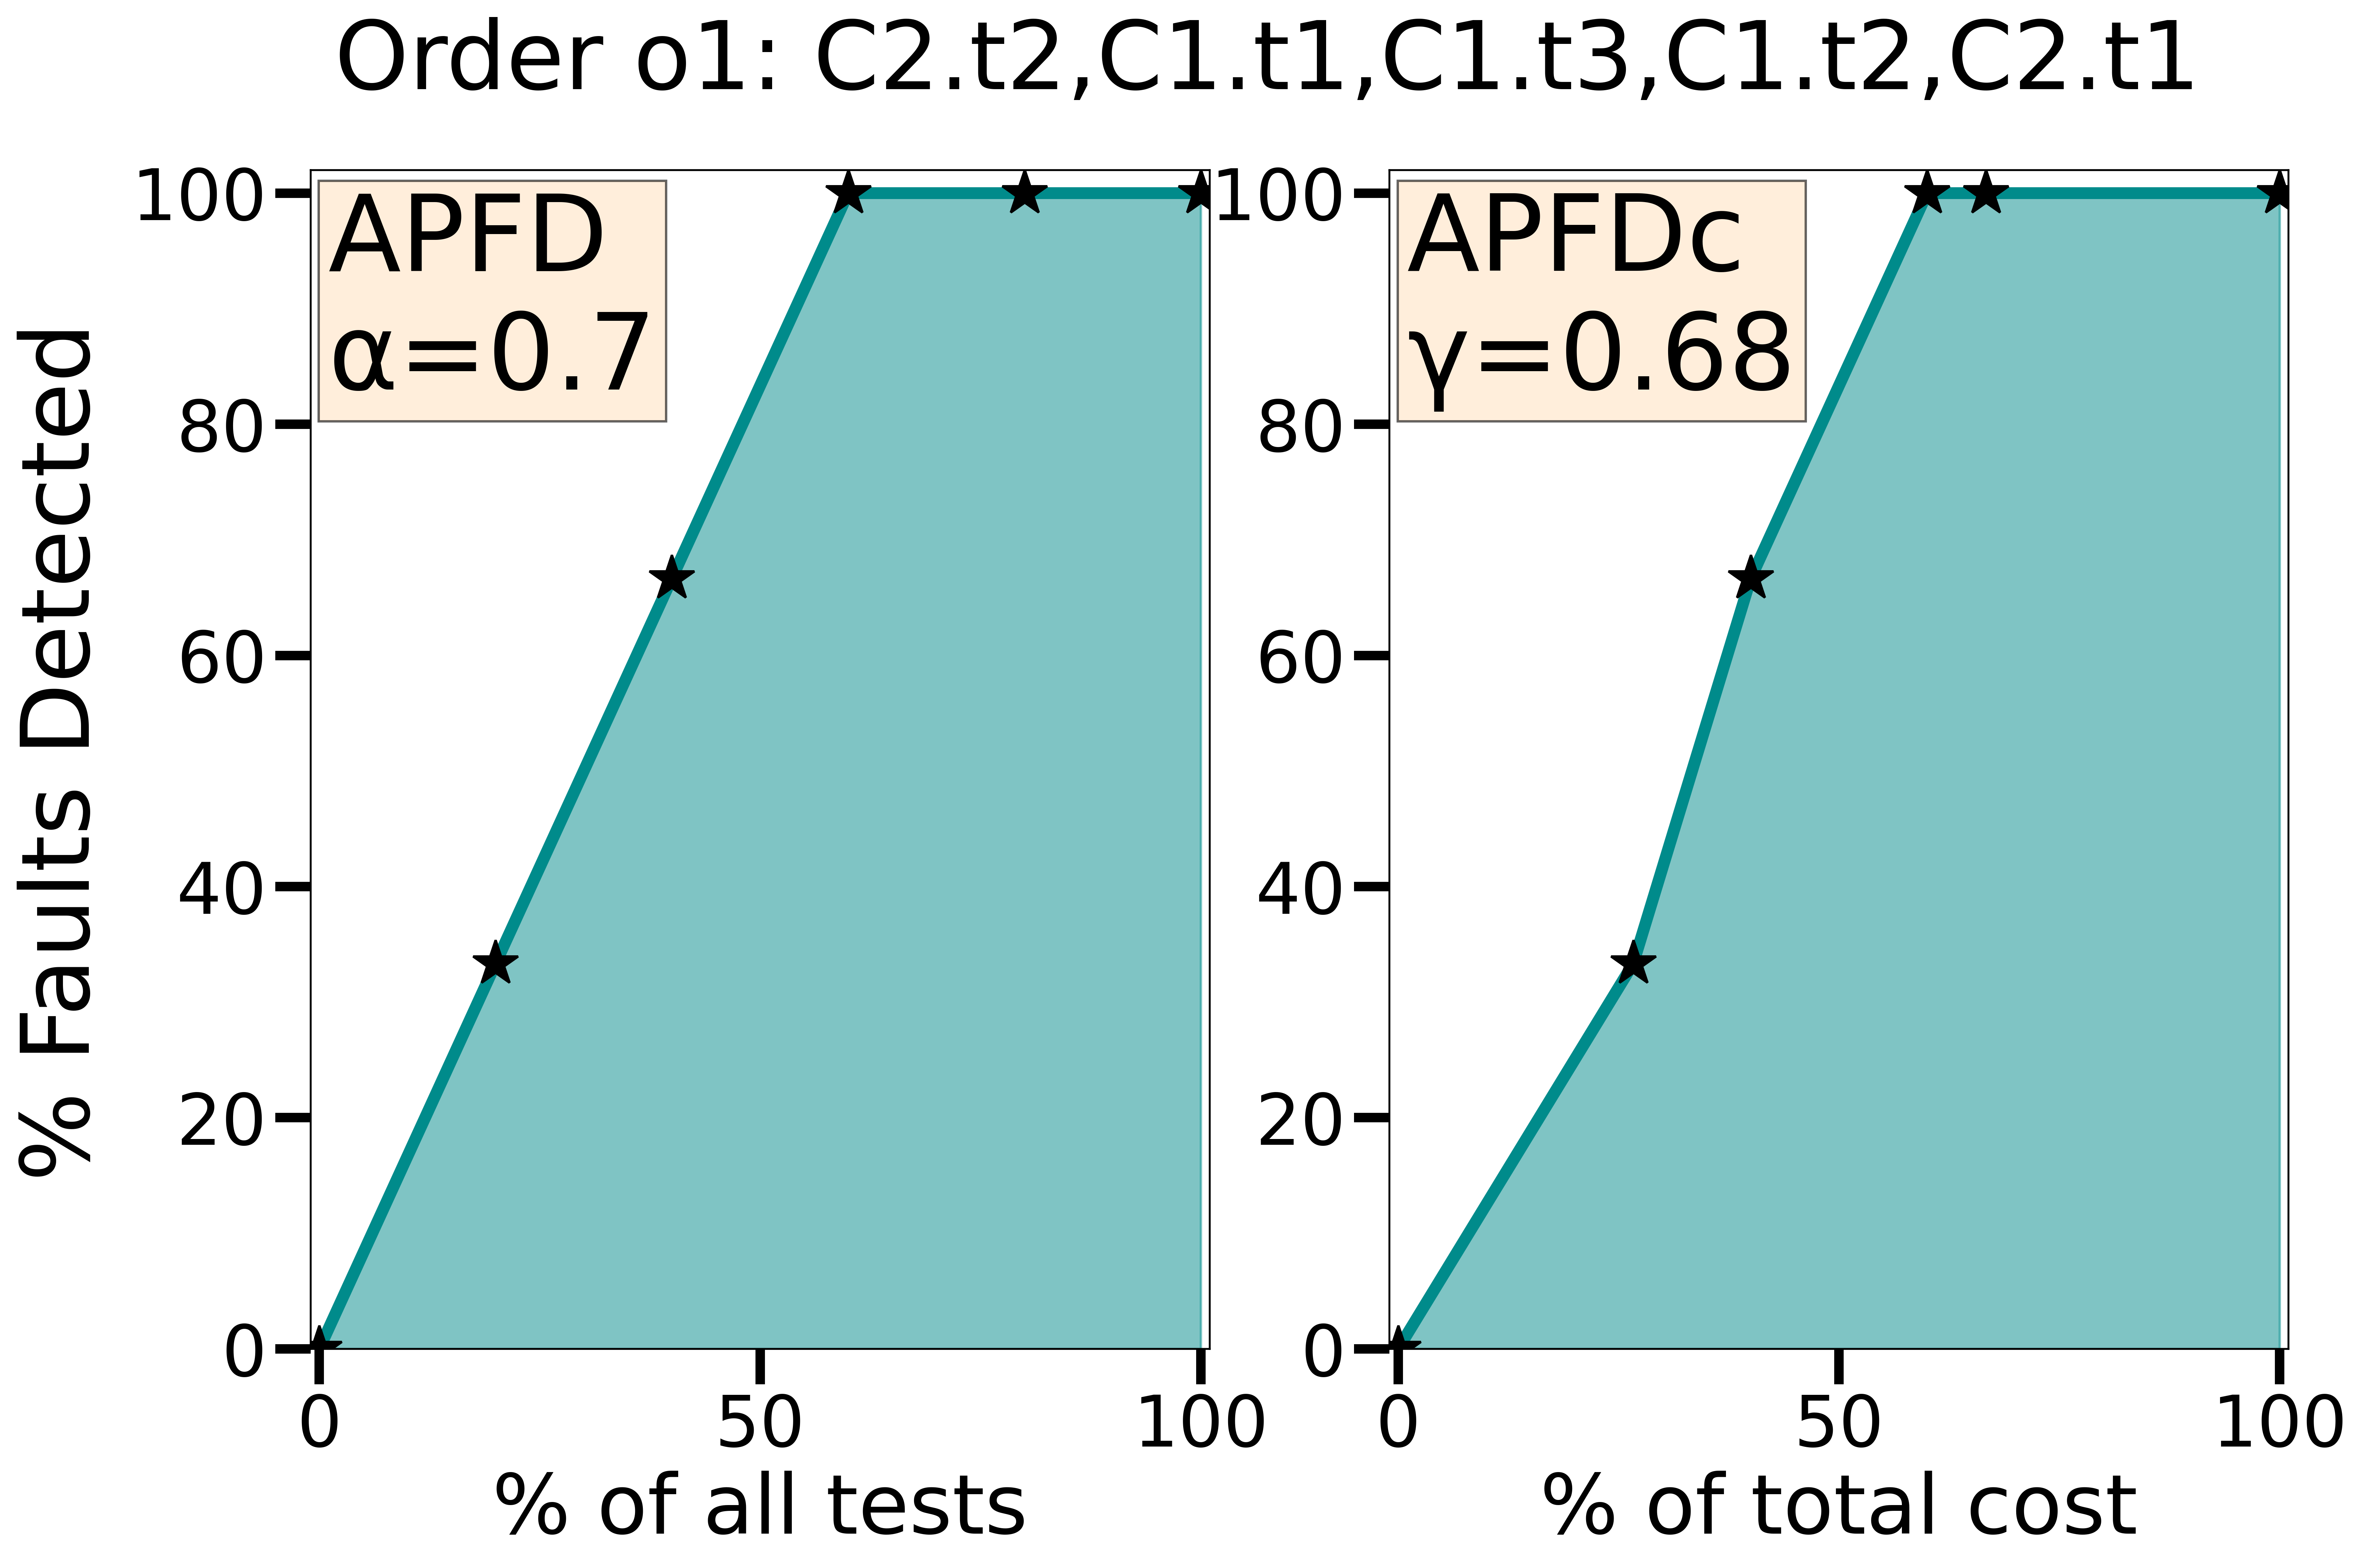
\includegraphics[width=\textwidth]{figures/5-1-3-2-4.png}
	\end{subfigure}
	\hfill
	\begin{subfigure}[b]{0.48\linewidth}
		\centering
		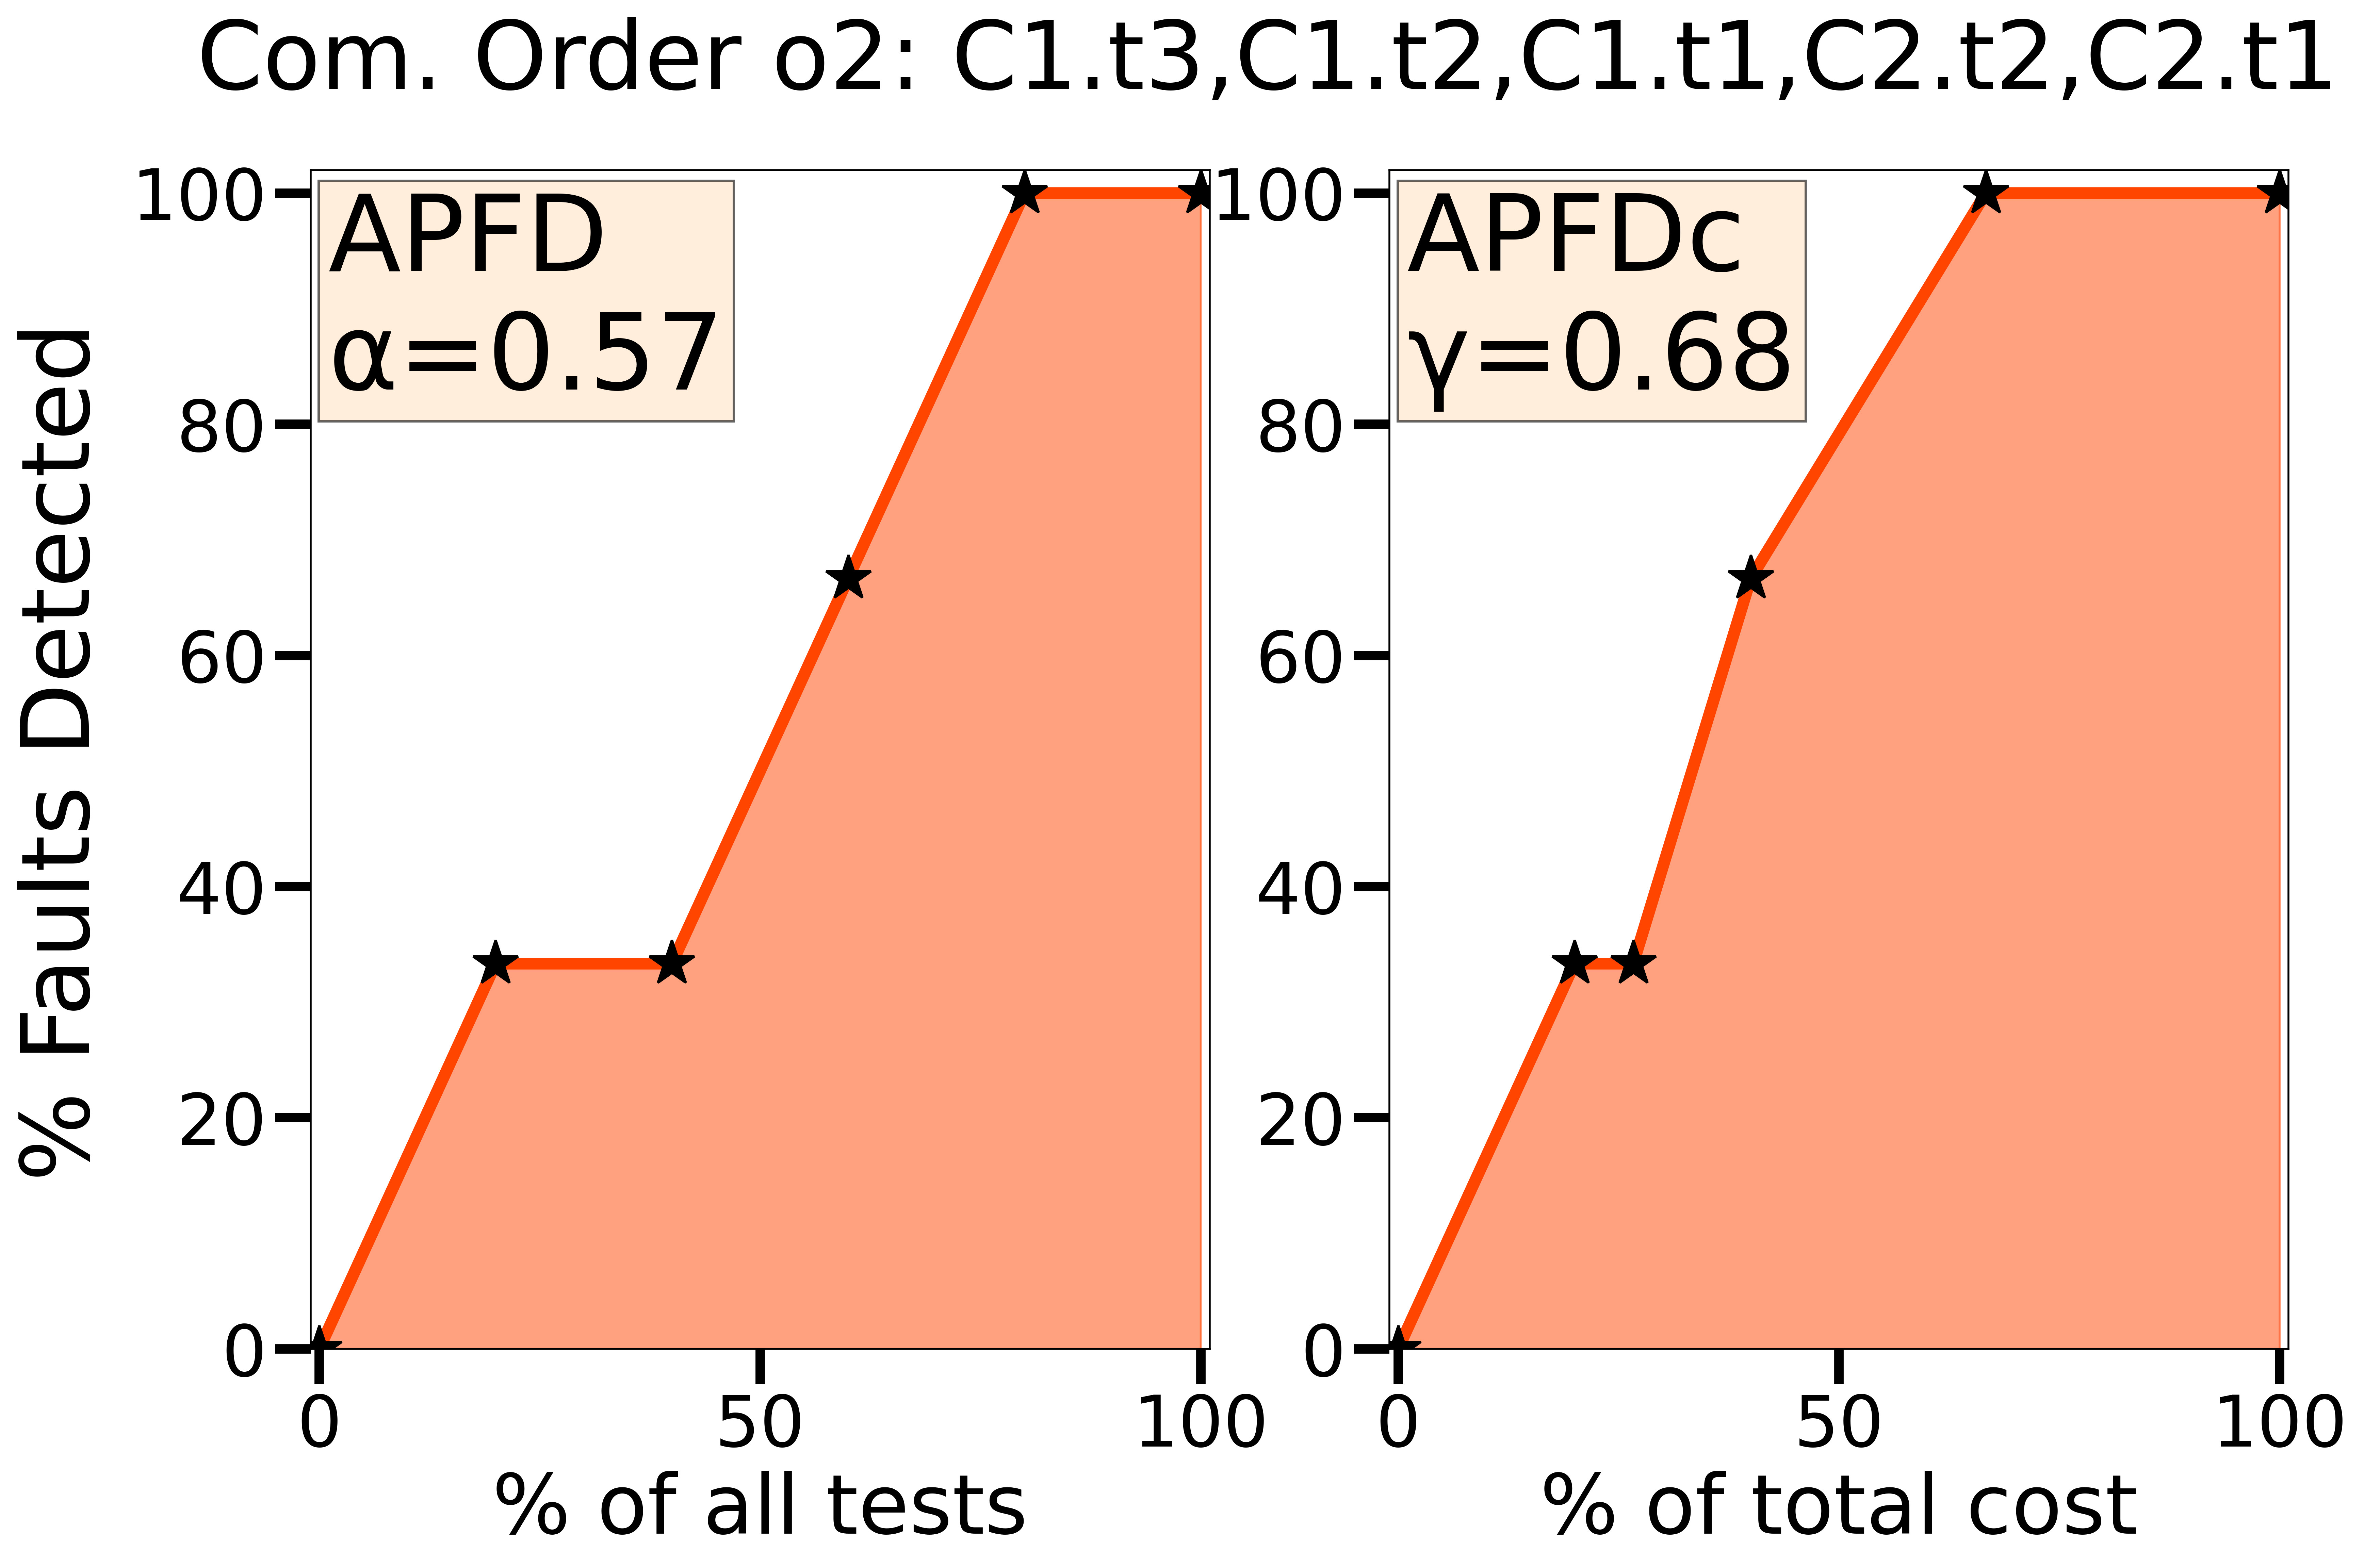
\includegraphics[width=\textwidth]{figures/3-2-1-5-4.png}
	\end{subfigure}
	\vspace{-1em}
	\caption{Example metrics for two orders (Com.\ is \compatible) for $n=5,m=3$; class C1 has 3 tests with costs $\langle40,20,60\rangle$, class C2 has 2 with $\langle100,80\rangle$; C1.t1 \detects fault F1; C1.t3 \detects F2; C2.t1 \detects F2 and F3; C2.t2 \detects F3.\label{fig:example}}
	\vspace{-0.2in}
\end{figure}

我们的记号很大程度上与提出\APFDFull{} (\APFD{})~\cite{rothermel2001prioritizing}和\APFDcFull{} (\APFDc{})~\cite{elbaum2001incorporating}的工作一致, 但我们显式地定义了 \mappingMatrix{}。
我们用$n$标记测试用例的数量,用$m$标记被这$n$个测试用例的其中一些检测到的缺陷数量。
我们用$M$标记一个\mappingMatrix{},也就是一个$n\times m$的布尔矩阵,其中$M_{j,i}=\textrm{true}$当且仅当测试用例$j$的失败可以\detects 缺陷$i$,并且其中每个缺陷都至少被一个测试用例检测(也就是说$\forall i.\exists j. M_{j,i}$)。
我们用$T$测试用例集中测试用例组成的一个集合.
我们将可以\detect{}缺陷$i$的测试用例的集合记做$T_i$,也就是说$T_i=\{j|M_{j,i}\}$。
总的来说,对于$i\ne i'$,$T_i$和$T_{i'}$可以有交集, 因为一个失败的测试用例可以\detect{}多个缺陷.
失败的总数记做$k$,也就是说$k=|\{j|\exists i. M_{j,i}\}|$,同时我们用$k_i$标记$T_i$集合的大小,即$k_i=|T_i|$。

对于一个执行次序$o$($T$的一个排列),我们用$<_o$来比较两个测试用例$t$和$t'$在该执行次序中的位置。$t<_o t'$表示$t$在$o$中先于$t'$执行,而$t\le_o t'$表示$t=t'$或$t<_o t'$。
我们用$t_{j}(o)$来表示$o$中的第$j$个测试用例。
我们用$TF_{i}(o)=\min_j M_{t_{j}(o),i}$标记$o$中第一个检测到故障$i$的测试用例的位置。
之前的工作~\cite{elbaum2001incorporating,rothermel2001prioritizing}定义了指标\APFD{}和\APFDc{}(使用符号$TF$而不是$\TF$)。
我们用$\APFD{}(o)$和$\APFDc{}(o)$分别表示执行次序$o$的 \APFD{}和\APFDc。
当从上下文可以清楚地知道所指的执行次序时,我们在$<_o$, $\le_o$, $t_{j}(o)$, $\TF_{i}(o)$, $\APFD{}(o)$, 和$\APFDc{}(o)$中省略$o$。

被使用最多的RTP指标是\APFD{}~\cite{rothermel2001prioritizing}。对一个执行次序$o$,\APFD{}定义如下。

\begin{mydefinition}[\APFD]
\APFDFull{}的定义为
\begin{equation}\label{definition_apfd}
    \APFD=1-\frac{\sum_{i=1}^m\TF_i}{nm}+\frac{1}{2n}
\end{equation}
\end{mydefinition}

如图~\ref{fig:example}中的两个例子所示,将检测到的缺陷百分比与执行的测试用例百分比作图,\APFD{}代表曲线下的面积。
图中每个点表示执行完若干测试用例后的情况,点之间的连线使得\APFD{}的均值/中位数具有良好的性质,并使其分布在一些情况下具有对称性(Section~\ref{sec:lit:review})。
\APFD{}的范围在0和1之间,更确切地说,在$1/(2n)$和$1-1/(2n)$之间。
较大的APFD{}表明一个测试用例平均而言较早检测到各个故障。

虽然\APFD{}有效地考虑了测试的数量,但 “代价感知型"指标\APFDc{}考虑了运行测试用例的代价~\cite{elbaum2001incorporating}。
运行测试用例的代价可以通过各种方式来衡量,但大多数工作都使用测试用例的运行时间。
我们用$\Cost{t}$表示一个测试用例$t$的代价(运行时间);一组测试$T$的总成本是$\Cost{T}=\sum_{t\in T}\Cost{t}$。

\begin{mydefinition}[\APFDc]
\APFDcFull{}的定义为
\begin{equation}\label{definition_apfdc}
    \APFDc=\frac{\sum_{i=1}^m\left(\sum_{j=\TF_i}^n\Cost{t_j}-\frac{1}{2}\Cost{t_{\TF_i}}\right)}{m\multi \Cost{T}}
\end{equation}
\end{mydefinition}

如\Figure~\ref{fig:example}所示,将检测到的缺陷百分比与测试用例集的总成本的百分比作图,\APFDc{}则代表曲线下的面积。
请注意,\APFD{}可以被看作是\APFDc{}在$\forall t,t’\in T.\Cost{t}=\Cost{t'}$情况下的一个特例。

在实践中,测试用例会被开发者分区,通常一个测试用例从属于一个\emph{\classes}——例如,JUnit~\cite{2021JUnit}中测试方法从属于测试类,Maven~\cite{2020Maven}中测试类属于测试模块,pytest~\cite{2021pytest}中测试函数属于测试文件--每个\class{}的测试一起运行。
我们之前的工作~\cite{wei2021probabilistic}将 \emph{\compatible{}}执行次序定义为每个\class{}的所有测试用例都是连续执行的执行次序。
我们用$T_\testClassInFormula$来表示$\testClassInFormula$\class{}中的测试用例的集合。
如果$\forall \testClassInFormula,j\le j'\le j''.t_{j}(o)\in T_\testClassInFormula\wedge t_{j''}(o)\in T_\testClassInFormula\Rightarrow t_{j'}(o)\in T_\testClassInFormula$,那么一个测试用例执行次序$o$是\compatible{}的。
例如,在\Figure~\ref{fig:example}中$o2$是\compatible{}的,而$o1$不是。

我们在不同的\emph{测试场景}中分析RTP技术,每个测试场景包含一个有$n$个测试用例、$m$个故障的测试用例集、\mappingMatrix{}、每个测试用例的代价以及对于$\consecutivetorders$每个测试的\class{}。
为了分析\compatible{}测试用例执行次序,我们引入一些新的符号来表示测试的\class{}。
我们用$T_{i,\testClassInFormula}=T_i\cap T_\testClassInFormula$来表示$\testClassInFormula$\class{}中能检测到$i$故障的测试集合。
我们用$\classSet$表示所有\class{}的集合,$\classSet_i$表示包含至少一个能检测到缺陷$i$的测试用例的\class{}的集合,即$\classSet_i=\{\testClassInFormula\in \classSet| T_{i,\testClassInFormula}\ne \emptyset\}$。
我们用$\classOfTest{t}$标记$t$所属的类,即$t\in T_{\classOfTest{t}}$。
\compatible{}测试用例执行次序的数量为$|\consecutivetorders|=|\classSet|!\prod_{\testClassInFormula\in \classSet}|T_\testClassInFormula|!$。

对于一组执行次序$S$,不管是$\alltorders$还是$\consecutivetorders$,RTP指标(\APFD{}或\APFDc{})的概率质量函数(\distribution{})是一个从指标值到其概率的函数$p$。$p(x)=\Prob{\mathrm{metric}=x}=\inlinefrac{|\{o\in S|\mathrm{metric}(o)=x\}|}{|S|}$。
所有先前的RTP工作都只显示了随机采样得到的随机RTP的样本分布,我们接下来推导一些\distributions{}。
\chapter{\APFD{}的\Distribution}

为了分析指标\APFD{}的\distribution{}。
我们首先提出一个算法来计算一般情况的$M$下的\APFD{}的\distribution{},然后我们讨论两个特殊情况,即最近RTP研究中最常见的\mappingAllToOne{}\mappingMatrices{}和\mappingOneToOne{}\mappingMatrices{}。

\section{一般情况下计算\APFD{}的\Distribution{}的算法}\label{sec:dpalgorithm}

为了计算\APFD{}的\distribution{},一个朴素的算法会将列举所有$n!$测试用例执行次序,并为每个执行次序计算\APFD{}。
理论上,\APFD{}最多可以取$O(n!)$不同的值,例如,当$m=\sum_{i=1}^nn^i$并且所有$n$个测试用例失败,并且分别\detect 到$n,n^2,\ldots,n^n$个不同的缺陷时,$n!$中的每个执行次序都有一个不同的\APFD{}。
然而,在实践中,缺陷的数量$m$和失败的数量$k$通常很小,例如,在我们的实验数据集~\cite{Peng2020IRTCP}中,2980个(98\%)\job{}中的2906个有$k\le 10$。
我们提出了一种算法,以$O(n^2mk\multi k!)$的时间复杂度计算精确的\distribution{}。
尽管有其中包含$k!$的项,该算法在实践中的运行时间是合理的,对于2906个\job{}中的任何一个都在30秒以内运行结束。
当$k>10$时,我们可以采用抽样的方法。

接下来我们描述一下我们算法的直觉。
$sum_{i=1}^m\TF_i$是\APFD{}中唯一依赖于测试用例执行次序的项,所以我们首先计算这个项的分布,然后将其转换为\APFD{}的分布。
枚举所有的缺陷求和并不能为其带来一个好的递归公式。
我们算法的关键是,将其转化为\emph{枚举$k$个失败测试用例的位置求和}。
我们把$sum_{i=1}^m\TF_i$看作是一个\emph{加权和}。
\begin{equation}\label{TF:weighted:sum}
\sum_{i=1}^m\TF_i=\sum_{j=1}^kw_j\position_j
\end{equation}
其中$\position_j$是执行次序中第j个失败测试用例的位置,$w_j\ge 0$是权重,其计算方式为第$j$个失败测试用例检测到的缺陷数量(算法~\ref{algo:distribution:APFD}的第~\ref{w_i:define}行)。
例如,考虑一下图~\ref{fig:example}中的测试用例执行次序$o1$。
$k=4$个失败测试用例的\emph{相对顺序}是$\relativeOrder=\langle\mathrm{C2.t2,C1.t1,C1.t3,C2.t1}\rangle$;我们使用记号$\relativeOrder$来区别于所有$n$个测试用例的执行次序的记号$o$。
对于这个相对顺序,$w=\langle 1,1,1,0\rangle$,因为$m=3$个缺陷首先由$\mathrm{C2.t2}$、$\mathrm{C1.t1}$和$\mathrm{C1.t3}$检测到。
对应这个相对顺序$\relativeOrder$的$\position$是$\position=\langle 1,2,3,5\rangle$,因为$\relativeOrder$中的$4$个失败测试用例在执行次序$o1$中出现在这些位置。

对于$\position=\langle\position_1\ldots\position_k\rangle$,如果$1\le\position_1<\ldots<\position_k\le n$,我们称$\position$是\emph{合法}的。
$\position$和$w=\langle w_1\ldots w_k\rangle$都可以在不同的测试用例执行次序中变化。
虽然$\position$有$\binom{n}{k}$个有效值,但因为$w$只取决于$\relativeOrder$,我们注意到$w$最多有$k!$个可能值(在实践中$k!\ll \binom{n}{k}$,因为$k\ll n$)。
因此,我们首先通过枚举$k$个失败测试用例的$k!$种相对顺序来固定$w$。
然后对于每种相对顺序,计算$\sum_{i=1}^m\TF_i=\sum_{j=1}^kw_j\position_j$的\distribution{}问题等价于\emph{“给定$w$,计算对于每个$s$使得$\sum_{j=1}^kw_j\position_j=s$的有效$\position$的数量"}。这个问题这可以按以下方式递归解决。

\begin{algorithm}[t]
\renewcommand\baselinestretch{0.9}\selectfont
\caption{计算\APFD{}的\distribution}
\label{algo:distribution:APFD}
\textbf{Input:} n,m,M \ccc{测试用例和缺陷的数量, 以及\mappingMatrix{}}\\

\textbf{Output:} $\Output$ \ccc{\APFD{}的\distribution{}: $\Output(x)=\Prob{\APFD{}=x}$}\\

\SetKwFunction{FMain}{PMF}
\SetKwProg{Fn}{Function}{}{}
\Fn{\FMain{}\emph{\ccc{主函数; 返回\APFD{}对所有测试用例执行次序的\distribution{}}}}{
    k = $\mathrm{|\{j|\exists i.\twoParaFunc{M}{j}{i}\}|}$ \ccc{M中失败的数量, 实践中k$\ll$n}\\
    q = \FuncSty{PMF\_sum()} \ccc{计算$\sum_{i=1}^m\TF_i$的\distribution}\\
    \KwRet{$\mathrm{\lambda x.q(mn-mnx+\frac{m}{2})}$} \ccc{将$\sum_{i=1}^m\TF_i$的\distribution{}转化为\APFD{}的\distribution{}}
}

\SetKwFunction{FMain}{PMF\_sum}
\SetKwProg{Fn}{Function}{}{}
\Fn{\FMain{}\emph{\ccc{return the \distribution of $\mathrm{\sum_{i=1}^m\TF_i}$ for all orders}}}{
    $\mathcal{P}$ = $\langle$\FuncSty{PMF\_rorder($\relativeOrder$)}$,\forall \relativeOrder \in perms(\{j|\exists i.\twoParaFunc{M}{j}{i}\})\rangle$ \ccc{枚举所有的相对位置}\label{line:enumerate:o}\\
    \KwRet{$\mathrm{\lambda x.\sum_{p\in \mathcal{P}}p(x)/|\mathcal{P}|}$} \ccc{将每种相对位置的$\sum_{i=1}^m\TF_i$的\distributions{}做平均}
}

\SetKwFunction{FMain}{PMF\_rorder}
\SetKwProg{Fn}{Function}{}{}
\Fn{\FMain{$\mathrm{\relativeOrder}$}\emph{\ccc{返回对于一种相对位置$\mathrm{\relativeOrder}$,$\mathrm{\sum_{i=1}^m\TF_i}$的\distribution{}}}}{
    w = $\langle | \{ i | \twoParaFunc{M}{\relativeOrder_j}{i}  \wedge \nexists j'<j. \twoParaFunc{M}{\relativeOrder_{j'}}{i}\} |, \forall j \in 1..k \rangle$
    \ccc{$\mathrm{w}$是公式\ref{TF:weighted:sum}中的权重}\label{w_i:definition}
    \\
    \KwRet{$\lambda s.$\FuncSty{f($\mathrm{w,k,n}$)}$(s)/\binom{n}{k}$} \ccc{$\position$的总共可能取值有$\binom{n}{k}$个}
}

\ccc{下面的函数应该被记忆化,以避免对重复的w,\paramOneInF,和\paramTwoInF{}组合重复计算}\\

\SetKwFunction{FMain}{f}
\SetKwProg{Fn}{Function}{}{}
\Fn{\FMain{$\mathrm{w,\paramOneInF,\paramTwoInF}$}\emph{\ccc{给定w,用公式\ref{f:recursive:equation}计算并返回$\mathrm{f_{\paramOneInF,\paramTwoInF}}$}}}{ 
    \uIf{$\mathrm{\paramOneInF>\paramTwoInF}$}{
        \KwRet{$\mathrm{\lambda s.0}$}
    }
    \uIf{$\mathrm{\paramOneInF=0}$}{
        \KwRet{$\mathrm{\lambda s.\mathbf{1}_{s=0}}$}
    }
    \KwRet{$\lambda s.$\FuncSty{f($\mathrm{w,\paramOneInF,\paramTwoInF-1}$)}$\mathrm{(s)+}$\FuncSty{f($\mathrm{w,\paramOneInF-1,\paramTwoInF-1}$)}$\mathrm{(s-w_{\paramOneInF}\paramTwoInF)}$}
}
\end{algorithm}


我们用$f_{\paramOneInF,\paramTwoInF}(s)$表示满足$1\le \position_1< \ldots < \position_{\paramOneInF}\le \paramTwoInF$且$\sum_{j=1}^{\paramOneInF}w_j\position_j=s$的情况下,$\position_1,\ldots,\position_{\paramOneInF}$的可能取值数量。那么我们要解决的问题就是求出$f_{k,n}(s)$。
作为基础情况,
(1)~$\paramOneInF>\paramTwoInF$时$f_{\paramOneInF,\paramTwoInF}(s)=0$,因为$\position_{\paramOneInF}<\paramOneInF$不可能成立。
(2)~$f_{0,\paramTwoInF}(s)=\mathbf{1}_{s=0}$,其中$\mathbf{1}$是指示函数,因为只有空序列$\langle\rangle$是合法的,并且$\sum_{j=1}^0w_j\position_j=0$。
对于所有$\paramTwoInF\ge \paramOneInF>0$,$f_{\paramOneInF,\paramTwoInF}(s)$的可能取值数有两种情况。(1)~如果$\position_{\paramOneInF}\le \paramTwoInF-1$,根据定义,这个数等于$f_{\paramOneInF,\paramTwoInF-1}(s)$。(2)~如果$\position_{\paramOneInF}=\paramTwoInF$,$s$的可能数量等于满足$\position_{\paramOneInF-1}\le \position_{\paramOneInF}-1= \paramTwoInF-1$和$\sum_{j=1}^{\paramOneInF-1}w_j\position_j=(\sum_{j=1}^{\paramOneInF}w_j\position_j)-w_{\paramOneInF}\position_{\paramOneInF}=s-w_{\paramOneInF}\paramTwoInF$的情况下$\position_1,\ldots,\position_{\paramOneInF-1}$的可能取值数,也就是$f_{\paramOneInF-1,\paramTwoInF-1}(s- w_{\paramOneInF}\paramTwoInF)$。
总的来说,我们有
\begin{equation}\label{f:recursive:equation}
f_{\paramOneInF,\paramTwoInF}(s)=\left\{
\begin{array}{lc}
0 & \quad\paramOneInF>\paramTwoInF\\
\mathbf{1}_{s=0} & \quad\paramOneInF=0\\
f_{\paramOneInF,\paramTwoInF-1}(s)+f_{\paramOneInF-1,\paramTwoInF-1}(s-w_{\paramOneInF}\paramTwoInF) & \quad\mathrm{其它情况}
\end{array}
\right.
\end{equation}
在解出$f_{k,n}$之后,我们得到了对于每种失败测试用例的相对位置的$\sum_{i=1}^m\TF_i$的\distribution{}。
根据对称性,$k!$种相对顺序都有相同的概率取到,因此我们只需这些\distributions{}的平均,就可以得到对所有测试用例执行次序的$\sum_{i=1}^m\TF_i$的\distribution{}。
最后,我们将$\sum_{i=1}^m\TF_i$的\distribution{}转换为\APFD{}的\distribution{}。


接下来我们更详细地描述算法~\ref{algo:distribution:APFD}。
输入是测试用例的数量$n$,缺陷数$m$,以及 \mappingMatrix{}$M$。
主函数\FuncSty{PMF}调用\FuncSty{PMF_sum}来获得 $\sum_{i=1}^m\TF_i$ 的\distribution{},并将其转换为\APFD{} 的\distribution{}。
函数\FuncSty{PMF\_sum}枚举$k$个失败测试用例的所有相对顺序$\relativeOrder$,调用\FuncSty{PMF\_rorder($\mathrm{\relativeOrder}$)}来获得每个相对顺序的$\sum_{i=1}^m\TF_i$的\distribution{}。并对这些\distributions{}进行平均,得到对所有(相对)执行次序的$\sum_{i=1}^m\TF_i$的分布。
函数\FuncSty{PMF\_rorder($\mathrm{\relativeOrder}$)}计算公式(\ref{TF:weighted:sum})中的权重$w$,调用 \FuncSty{f(w,k,n)}以得到对于$w$的$f_{k,n}$,并将其转换为$\sum_{i=1}^m\TF_i$的\distribution{}。

我们最后讨论算法~\ref{algo:distribution:APFD}的时间复杂度和实践中的性能。
算法的主要的运行成本来自于计算函数\FuncSty{f}。
因为有$O(k!)$种不同的$w$和$0\le \paramOneInF\le k,\paramOneInF\le \paramTwoInF\le n$,我们要为$O(nk\multi k!)$种不同的输入计算\FuncSty{f}。
通过记忆化,对每种输入只需计算一次\FuncSty{f}。
每次计算需要$O(nm)$,因为$|\mathrm{support}(f_{\paramOneInF,\paramTwoInF})|=O(nm)$(对于每个$1\le i\le m$,我们有$1\le \TF_i\le n$)。
 因此,对所有输入计算\FuncSty{f}的成本是$O(n^2mk\multi k!)$。
算法中的其他成本低于\FuncSty{f}的成本;因此,算法~\ref{algo:distribution:APFD}的总体时间复杂度为$O(n^2mk\multi k!)$。

\newcommand{\mysubsubsection}[1]{\noindent\textbf{#1:}}
\mysubsubsection{实现}
虽然自上而下的递归使算法展示起来更清楚,但为了获得更好的性能,我们的实现使用自下而上的动态规划来计算\FuncSty{f}。
我们的实现只使用了\CPPLine{}行的C++代码。

\mysubsubsection{数据集}
我们使用拥有最多Java项目的RTP数据集~\cite{Peng2020IRTCP}对算法进行评估。
在这个数据集中,每个测试用例是一个测试类,每个\class{}是一个Maven模块~\cite{2020Maven}。
该数据集有2980个\job{},其中2906个(98\%)有$k\le 10$。
对于每个$k\le 10$,我们从数据集中选择具有最大测试用例数量($n$)的\job{}。
我们还合成了一个有2118(数据集中最大的测试用例数)个测试用例、10个失败的虚拟\job{}。
我们在所选的\job{}上使用了\mappingAllToOne{}和 \mappingOneToOne{}的\mappingMatrices{}。

\begin{table*}[t]
\centering
\vspace{-1em}
\caption{对于10个最大的\job{}~\cite{Peng2020IRTCP}和一个合成\job{} (TSmax),测试用例的数量, 失败的数量,算法运行时间(单位ms),和Jensen-Shannon(JS)距离}
\label{tab:numbersforjobs}
\begin{tabular}{|l||r|r|r|r||r|}
\hline
\multicolumn{1}{|c||}{\textbf{Test}} & \textbf{\#Tests} & \textbf{\#Failures} & \multicolumn{2}{c||}{\textbf{Runtime [ms]}}& \textbf{Jensen-Shannon}  \\
\multicolumn{1}{|c||}{\textbf{suite}} & \multicolumn{1}{c|}{\textbf{$(n)$}} & \multicolumn{1}{c|}{\textbf{$(k)$}} & \textbf{\mappingAllToOne} &\textbf{\mappingOneToOne} & \multicolumn{1}{c|}{\textbf{distance} (\S3.2.2)} \\
\hline
TS1 & 2118 & 1  & 513& 505 & 0.0000\\
TS2 & 1986 & 2   & 563& 629& 0.0005\\
TS3 & 2080 & 3   & 617& 871& 0.0003\\
TS4 & 1929 & 4   & 680& 1147& 0.0004\\
TS5 & 1795& 5&  731&1408& 0.0006\\
TS6 & 339& 6&  627&732& 0.0040\\
TS7 & 465& 7&  678&756& 0.0034\\
TS8 & 813& 8 & 829&2009&  0.0023\\
TS9 & 52& 9&  1496 &1846& 0.0442\\
TS10& 161 & 10&  10989 &27095& 0.0150\\
\hline
TSmax & 2118& 10&  32801 &242400& 0.0011\\
\hline
\end{tabular}
\end{table*}


\mysubsubsection{评估}
如\Table~\ref{tab:numbersforjobs}所示,对于所有真实的\job{},代码在30秒内运行结束(在一台普通的笔记本电脑上);对于合成的\job{},在\mappingAllToOne{}和\mappingOneToOne{}的情况需要更多时间,但仍分别只用了33秒和4分钟。

\section{特殊情况下\APFD{}的\Distributions{}}

我们在Section~\ref{sec:introduction}中提到,最近的RTP研究使用了真实的失败和缺陷,使用了两种\mappingMatrices{}:\mappingAllToOne{}和\mappingOneToOne{}。
我们接下来讨论这两种常用情况下的\APFD{}的\distributions{}。

\noindent\textbf{\allToOneSec{} \mappingAllToOne{}:}
我们首先为\mappingAllToOne推导出\APFD{}的\distribution{}。
在这种情况下,$m=1$,$k\ge 1$,在公式~(\ref{TF:weighted:sum})中$w_1=1,\forall j>1.w_j=0$。
因此,对于$\paramOneInF>1$,递归公式~(\ref{f:recursive:equation})变成$f_{\paramOneInF,\paramTwoInF}(s)=f_{\paramOneInF,\paramTwoInF-1}(s)+f_{\paramOneInF-1,\paramTwoInF-1}(s)$,这与帕斯卡三角形形式相似。
这一观察提示我们,对于\mappingAllToOne{}的 \APFD{}的\distribution{}可能有一个带有二项式系数的封闭解。

\begin{mytheorem}[\mappingAllToOne{}\mappingMatrixThe{}情况下\APFD{}的\distribution{}]\label{distribution-apfd-one2one}
\begin{equation}\label{formula-distribution-apfd-one2one}
    \Prob{\APFD{}= 1-\frac{s}{n}+\frac{1}{2n}}=\frac{\binom{n-s}{k-1}}{\binom{n}{k}},s\in\{1,2,\ldots,n-k+1\}
\end{equation}
\end{mytheorem}
\begin{proof}
对于\mappingAllToOne{},\APFD{}值仅取决于$\TF_1$,这本质上是公式~(\ref{\TF:weighted:sum})中的$\position_1$。
对于$1\le s\le n-k+1$,只要$s=\position_1<\ldots<\position_k\le n$,$\TF_1=s$就成立。
为了满足这个条件,我们只需要在位置$s$之后选择$k-1$个位置。
因此,在$\binom{n}{k}$种从$n$个位置中选$k$个位置的方法中有$\binom{n-s}{k-1}$个满足条件,所以$\Prob{\TF_1= s}=\inlinefrac{\binom{n-s}{k-1}}{\binom{n}{k}}$,公式(\ref{formula-distribution-apfd-one2one})可以由此直接得出。
\end{proof}

通过\formula{formula-distribution-apfd-one2one},我们可以用$O(n)$的时间来计算\APFD{}在\mappingAllToOne{}情况下的\distribution{}。
我们可以从$\binom{k-1}{k-1}=1$开始,用递推公式$\binom{n'+1}{k-1}=\frac{n'+1}{n'-k+2}\binom{n'}{k-1}, n'\ge k-1$,迭代计算所需的二项系数,得到$\binom{n}{k}=\frac{n}{k}\binom{n-1}{k-1}$。

\noindent\textbf{\oneToOneSec{} \mappingOneToOne{}:} 我们接下来考虑\mappingOneToOne{}下\APFD{}的\distribution{}。
在这种情况下,$m=k$,每个失败的测试用例都会发现一个不同的缺陷,所以对于每种$k$个失败测试用例的相对顺序,在公式(\ref{TF:weighted:sum})中有$\forall j.w_j=1$。
因此,运行算法~\ref{algo:distribution:APFD}并对$w$进行记忆化,复杂度变为$O(n^2k^2+k!)$。
$k!$的项来自于遍历所有的相对顺序。
如果我们事先检查\mappingMatrix{}是否为\mappingOneToOne{},我们就可以避免$k!$的项,所以复杂度是$O(n^2k^2)$。

此外,考虑到当$\forall j.w_j=1$时的公式(\ref{f:recursive:equation}),$f_{k,n}$本质上建模了这样的问题:\emph{“计算将整数$s$拆分成$k$个$\{1,2,\ldots,n\}$中不同的整数相加的情况数量”}。
具体来说,$f_{\paramOneInF,\paramTwoInF}(s)$可以被看作将$s$拆分成$\paramOneInF$个$\{1,2,\ldots,\paramTwoInF\}$中不同整数相加的情况数量。
我们有$f_{\paramOneInF,\paramTwoInF}(s)=f_{\paramOneInF,\paramTwoInF-1}(s)+f_{\paramOneInF-1,\paramTwoInF-1}(s-\paramTwoInF)$,因为拆分出的第$\paramOneInF$个整数或是小于$\paramTwoInF$或是等于$\paramTwoInF$,这两种情况分别对应$f_{\paramOneInF,\paramTwoInF-1}(s)$和$f_{\paramOneInF-1,\paramTwoInF-1}(s-\paramTwoInF)$。
据我们所知,这个问题没有已知的封闭解。
考虑到在我们的评估数据集中,99.8\%(2975/2980)的测试场景有$n^2k^2< 10^9$,$O(n^2k^2)$算法对于几乎所有实际情况是足够高效的。

\noindent\textbf{近似解:} 此外,我们可以通过忽略“不同数字”的约束来近似计算\distribution{},即:\emph{“计算将整数$s$拆分成$k$个$\{1,2,\ldots,n\}$中整数相加的情况数量”}。
这个问题有一个很简洁的生成函数$(x+x^2+\ldots+x^n)^k$,其中$x^s$的系数是拆分的数量~\cite{stanley2011enumerative}。
\begin{equation}\label{approximation:APFD:generating:function:coefficient}
    \sum_{i=0}^{\lfloor \frac{s-k}{n}\rfloor}\binom{k}{i}(-1)^i\binom{s-ni-1}{k-1}
\end{equation}
我们可以用两种不同的算法来计算这些系数。
第一种算法首先用帕斯卡尔三角法预计算二项式系数,然后用公式~(\ref{approximation:APFD: generating:function:coefficient})计算所有系数。
第一步需要$O(nk^2)$,因为$s-ni-1\le nk$和$i\le k$。
第二步需要$O(nk^2)$,因为每个$O(nk)$的系数需要$O(k)$来计算($\lfloor\frac{s-k}{n}\rfloor\le k$)。
因此,第一个算法的总体时间复杂度为$O(nk^2)$。
第二种算法直接用快速傅里叶变换~\cite{brigham1988fast}计算生成函数,其首先将$x+x^2+\ldots+x^n$转换为点值表示,将每个点值计算为第$k$次方,然后插值得到系数。
第二个算法需要$O(nk\log(nk))$,因为多项式的长度是$O(nk)$。
比较这两个算法的时间复杂度,当$k$与$n$相比很小时(即$k-\log k<\log n$),第一种算法更好,否则第二种算法更好。

我们用准确的\distribution{}和近似得到的\distribution{}之间的Jensen–Shannon(JS)距离~\cite{endres2003new}来评估我们的近似解。我们在与章节~\ref{sec:dpalgorithm}中相同的真实\job{}中评估了近似解。如表~\ref{tab:numbersforjobs}所示,我们的近似解具有较小JS距离,其中JS距离最大只有\Num{0.0442,($n=52,k=9$)}。

\section{\APFDc{}的\Distribution{}}

\APFDc{}的\distribution{}比\APFD{}的\distribution{}更复杂,因为即使是最简单的\mappingAllToOne{}\mappingMatrix{},\APFDc{}的可能值的数量可以是$\Omega(2^n)$。
例如,考虑$n$个测试用例,代价分别为$1,2,4,\ldots,2^{n-1}$,只有一个测试用例失败并且 \detects{}唯一的缺陷。
 \APFDc{}值取决于在执行次序中位于失败之前的测试用例的代价之和。
$2^{n-1}$种不同的测试用例的集合可以在失败之前,并且每一个集合都有不同的代价总和。
即使是对于\Figure~\ref{fig:example}中的例子,\APFDc{}(33)的支持集大小也比\APFD{}(8)大得多。

\chapter{考虑所有测试用例执行次序$\alltorders$时的期望值}\label{section:expected}

虽然有些RTP技术的比较使用了完整的样本\distribution{},但许多人只使用样本的算术平均值。
接下来我们推导出指标的期望值的公式,以更快地获得平均值,并且消除抽样的不精确性。
 
在这一章中,我们考虑从$\alltorders$中均匀随机选择一个执行次序$o$的情况,允许$n$测试用例的所有$n!$执行次序。
 因为\APFD{}是\APFDc{}在$\forall t,t'\in T.\Cost{t}=\Cost{t'}$时的一个特例,我们首先推导\APFDc{}的期望值。
 
我们从一个简单的例子开始,考虑一个只有一个失败测试用例的测试用例集($k=1$)。
对于一个随机顺序,该失败可以在任何位置,概率相同。
直观地说,对所有测试用例执行次序而言失败的平均位置是在序列的中间,因此,\APFD{}和\APFDc{}应该大约是$\half$。
事实上,我们将证明它们正好是$\half$。
此外,只要每个缺陷只被一个失败的测试用例\detect{}到($\forall i.k_i=|T_i|=1$,其中包括 \mappingOneToOne{}),那么 \APFD{}和\APFDc{}的期望值都是$\half$。
一般来说,\mappingMatrix{}可以更复杂:许多测试用例可以\detect{}同一缺陷,而一个测试用例可以\detect{}许多缺陷。
为了计算\APFD{}和\APFDc{}的期望值,我们首先证明一个有用的引理。

\begin{mylemma}\label{lemma:probability_precede_any}
对于每个缺陷$i$,
\begin{equation}\label{probability_precede_any}
\forall t\notin T_i.\Proba{t< t_{\TF_i}}=\Proba{\forall t'\in T_i.t< t'}=\frac{1}{k_i+1}
\end{equation}
\end{mylemma}
\begin{proof}
由于$\TF_i$是执行次序中来自$T_i$的第一个测试用例的位置,$t$先于$t_{\TF_i}$当且仅当$t$先于每个$t'\in T_i$。
考虑在一个随机执行次序中,每个$t\notin T_i$相对于$T_i$中所有测试用例的位置。
根据对称性,$t$前面有$T_i$的$0,1,\ldots,k_i$个测试用例的可能性是相同的。
因此,$t$处于$T_i$的所有$k_i$个测试用例之前的概率是$\frac{1}{k_i+1}$。
\end{proof}
我们首先用该引理来计算$\Ea{\APFDc}$。
\begin{mytheorem}[$\alltorders$中\APFDc{}的期望值]\label{theorem:expected:apfdc}
\begin{equation}\label{expected_apfdc}
\Ea{\APFDc}=1-\frac{\sum_{i=1}^m\left(\frac{\Cost{T\setminus T_i}}{k_i+1}+\frac{\Cost{T_i}}{2k_i}\right)}{m\multi \Cost{T}}
\end{equation}
\end{mytheorem}
\begin{proof}
由\formula{definition_apfdc},\APFDc{}中的两个关键项是$\Cost{t_{\TF_i}$和$\sum_{j=\TF_i}^n\Cost{t_j}$。
根据对称性,任何测试用例$t\in T_i$都可以以$frac1{k_i}$的概率是执行次序中的第一个,或者说$t=t_{TF_i}$。因此
\begin{equation}\label{apfdc_intermidiate1}
    \Ea{\Cost{t_{\TF_i}}}=\sum_{t\in T_i} \Prob{t = t_{\TF_i}}\Cost{t} = \frac{\Cost{T_i}}{k_i}
\end{equation}
接下来,考虑到$\sum_{j=\TF_i}^n\Cost{t_j}=\sum_{t\in T}\Cost{t}\mathbf{1}_{t_{\TF_i}\le t}$也可以按$\sum_{t\in T_i}\Cost{t}\mathbf{1}_{t_{\TF_i}\le t}+\sum_{t\notin T_i}\Cost{t}\mathbf{1}_{t_{\TF_i}\le t}$计算。
对于每个测试用例$t\in T_i$,根据定义,$t_{\TF_i}\le t$,所以$\forall t\in T_i.\Ea{\mathbf{1}_{t_{\TF_i}\le t}}=1$。
对于每一个测试用例$t\notin T_i$,有$\Ea{\mathbf{1}_{t_{\TF_i}\le t}}=\Proba{t_{\TF_i}\le t}=1-\Proba{t< t_{\TF_i}}=\frac{k_i}{k_i+1}$。
最后一个等式源于引理~\ref{lemma:probability_precede_any}。
因此,根据期望的线性,我们得到
\begin{equation}\label{apfdc_intermidiate2}
    \Ea{\sum_{j=\TF_i}^n\Cost{t_j}}=\Cost{T_i}+\frac{k_i}{k_i+1}\Cost{T\setminus T_i}
\end{equation}

从公式(\ref{definition_apfdc}),(\ref{apfdc_intermidiate1}),和(\ref{apfdc_intermidiate2}),我们得到\formula{expected_apfdc}。
\end{proof}
\begin{mycorollary}[$\alltorders$中\APFD{}的期望值]
\begin{equation}\label{expected_apfd}
    \Ea{\APFD}=1-\frac{(n+1)\sum_{i=1}^m \frac{1}{k_i+1}}{nm}+\frac{1}{2n}
\end{equation}
\end{mycorollary}
\ShowCorollaryProof{
\begin{proof}
在\formula{expected_apfdc}中令$\forall t,t'\in T.\Cost{t}=\Cost{t'}$即得到\formula{expected_apfd}.
\end{proof}
}
重新审视每个缺陷只能由一个失败的测试用例\detect{}的情况,在\formula{expected_apfdc}或\formula{expected_apfd}中令$\forall i.k_i=1$,正好给出$\half=\Ea{\APFD}=\Ea{\APFDc}$。
事实上,即使是在任何\mappingMatrix{}的一般情况下,我们也会发现这两个期望值很相似,这启发我们推导出以下不等式:
\begin{mytheorem}[$\alltorders$中\APFD{}和\APFDc{}的期望差异]\label{difference_with_interleaving}
\begin{equation}
    -\frac{1}{12}<\Ea{\APFD}-\Ea{\APFDc}<\frac{1}{2n}
\end{equation}
\end{mytheorem}
\begin{proof}
从公式(\ref{expected_apfdc})和(\ref{expected_apfd})中,我们有$\Ea{\APFD}-\Ea{\APFDc}=\Delta_{\APFDc{}}-\Delta_{\APFD{}}+\frac{1}{2n}$,其中$\Delta_{\APFDc{}}=\frac{\sum_{i=1}^m(\frac{1}{2k_i}-\frac{1}{k_i+1})\Cost{T_i}}{m\multi \Cost{T}}$以及$\Delta_{\APFD{}}=\frac{\sum_{i=1}^m\frac{1}{k_i+1}}{nm}$。
因为$k_i\ge 1$,我们有$-\frac{1}{12}\le\frac{1}{2k_i}-\frac{1}{k_i+1}\le 0$(使用基本微积分可以推导出,最小值在$k_i=2$或$k_i=3$时取到)。这一事实与$\Cost{T_i}\le \Cost{T}$结合,可以得出$-\frac{1}{12}\le \Delta_{\APFDc{}}\le 0$。
因为$k_i\ge 1$,我们也有$0<\frac{1}{k_i+1}\le \frac{1}{2}$,因而可以得出$0< \Delta_{\APFD{}}\le \frac{1}{2n}$。
因此,我们有$-\frac{1}{12}\le \Delta_{\APFDc{}}-\Delta_{\APFD{}}+\frac{1}{2n}< \frac{1}{2n}$。
然而,$\Delta_{\APFDc{}}-\Delta_{\APFD{}}+\frac{1}{2n}=-\frac{1}{12}$需要$\Delta_{\APFD{}}=\frac{1}{2n}$,因而$\forall i.k_i=1$,而在这种情况下$\Delta_{\APFDc{}}=0$以及$\Delta_{\APFDc{}}-\Delta_{\APFD{}}+\frac{1}{2n}=0\ne -\frac{1}{12}$。
因此,等号不能成立,所以$-\frac{1}{12}<\Ea{\APFD}-\Ea{\APFDc}<\frac{1}{2n}$。
\end{proof}

\chapter{考虑所有\Compatible{}测试用例执行次序$\consecutivetorders$时的期望值}

在这一节中,我们考虑$\consecutivetorders$中\APFD{}和\APFDc{}的期望值。
如第~\ref{sec:preliminaries}节所定义的,\cOmpatible{}测试用例执行次序不交错执行来自不同\class{}的测试用例。
与$\alltorders$类似,我们首先为$\consecutivetorders$证明一个有用的引理。

\begin{mylemma}\label{lemma:probability_precede_any:compatible}
对于每个缺陷$i$, (注意如果$t\notin T_i$, $C(t)$可能有另一个$t'\in T_i$) 
\begin{equation}\label{probability_precede_any:compatible}
\forall t\notin T_i.\Probn{t< t_{\TF_i}}=\Probn{\forall t'\in T_i.t< t'}=\left\{
\begin{array}{lc}
\frac{1}{|\classSet_i|(|T_{i,\classOfTest{t}}|+1)} & \quad\classOfTest{t}\in \classSet_i\\
\frac{1}{|\classSet_i|+1} & \quad\classOfTest{t}\notin \classSet_i
\end{array}
\right.
\end{equation}
\end{mylemma}
\begin{proof}
对于$\classOfTest{t}\in \classSet_i$的情况,为了使$t\notin T_{i,\classOfTest{t}}$排在所有能\detect{}缺陷$i$的测试用例之前,有两个条件必须成立。
首先,在$\classSet_i$中的所有\class{}中,$\classOfTest{t}$必须是第一个。根据对称性,$\classSet_i$中的每个\class{}都可以以相同的概率$\frac{1}{|classSet_i|}$成为第一个。
第二,$t$必须先于$T_{i,\classOfTest{t}}$的所有测试用例,(与引理~\ref{lemma:probability_precede_any}类似)以$\frac{1}{|T_{i,\classOfTest{t}}|+1}$的概率成立。
这两个条件是独立的,因为它们分别是关于\class{}的顺序和\class{}内的测试用例顺序,而这些顺序是相互独立的。
因此,$t$先于第一个\detect{}到缺陷$i$的测试用例的概率是$\frac{1}{|\classSet_i|(|T_{i,\classOfTest{t}|+1)}$。

对于$\classOfTest{t}\notin \classSet_i$的情况,只有一个条件——$\classOfTest{t}$先于$\classSet_i$中的所有\class{},就能使$t$先于第一个\detect{}到$i$的测试用例,这(与引理~\ref{lemma:probability_precede_any}相似)以概率$\frac{1}{|\classSet_i|+1}$发生。
\end{proof}

\begin{mytheorem}[$\consecutivetorders$中\APFDc{}的期望值]
\begin{equation}\label{expected_apfdc_no_interleaving}
\begin{array}{rl}
\En{\APFDc}=1-\frac{1}{m\multi \Cost{T}}\sum_{i=1}^m\Bigg(&\frac{\sum_{\testClassInFormula \notin \classSet_i}\Cost{T_\testClassInFormula}}{|\classSet_i|+1}+\\
    &\frac{1}{|\classSet_i|}\sum_{\testClassInFormula \in \classSet_i}\left(\frac{\Cost{T_\testClassInFormula \setminus T_{i,\testClassInFormula}}}{|T_{i,\testClassInFormula}|+1}+\frac{\Cost{T_{i,\testClassInFormula}}}{2|T_{i,\testClassInFormula}|}\right)\Bigg)
\end{array}
\end{equation}
\end{mytheorem}

% [ ADD FOLLOWING CHAPTERS HERE ]

\clearpage

\small
\linespread{1}\selectfont %正文,五号,中文宋体,英文Time new roman,1倍行距
\addcontentsline{toc}{chapter}{参考文献}
\bibliographystyle{bib/splncs04}
\bibliography{bib/references,bib/crossrefs}
\clearpage

\linespread{1.5}\selectfont\normalsize %正文,小四号,中文宋体,英文Time new roman,1.5倍行距
\chapter*{致谢}
\addcontentsline{toc}{chapter}{致谢}

感谢肖元安同学维护毕业论文的overleaf模板,这个模板大大减少了我的工作量。
\clearpage

\chapter*{北京大学学位论文原创性声明和使用授权说明}
\addcontentsline{toc}{chapter}{北京大学学位论文原创性声明和使用授权说明}
\input{head/honor}
\thispagestyle{empty}

\end{document}
